\section{Framework Scrum}
\begin{mdframed}
    \textbf{Scrum:} processo agile che nasce per lo sviluppo di progetti complessi, che ci permette di concentrarci sulla consegna del maggior valore business nel più breve tempo.
\end{mdframed}

\subsection{Caratteristiche}
\begin{itemize}
    \item Leggero
    \item Facile da capire
    \item Difficile da padroneggiare
\end{itemize}

\subsubsection{3 Pilastri}
\begin{itemize}
    \item \textbf{Trasparenza:} linguaggio comune per una conoscenza condivisa
    \item \textbf{Controllo:} ispezioni pianificate per prevenire variazioni non desiderate
    \item \textbf{Adattamento:} aggiustamenti per minimizzare ulteriori deviazioni tramite feedback continuo
\end{itemize}

\subsubsection{Proprietà}
\begin{itemize}
    \item Gruppi che si \textbf{auto-organizzano}
    \item Il prodotto evolve attraverso \textbf{sprint} di durata fissa
    \item I requisiti sono trattati come elementi di una lista detta “product backlog”
    \item Non vengono prescritte particolari pratiche ingegneristiche
    \item Si basa sull'attività empirica cioè la conoscenza si basa sull'esperienza e le decisioni si basano su ciò che è conosciuto
    \item \textbf{Processo iterativo e incrementale} per ottimizzare il controllo dello sviluppo e il controllo del rischio
\end{itemize}

\subsection{Sprint}
\begin{itemize}
    \item I progetti Scrum progrediscono attraverso una serie di sprint
    \item Durata tipica di 2-4 settimane: una durata costante favorisce un ritmo migliore
    \item Il prodotto è progettato, realizzato e testato durante lo sprint
\end{itemize}
\begin{center}
    \begin{tabular}{c}
        \\ 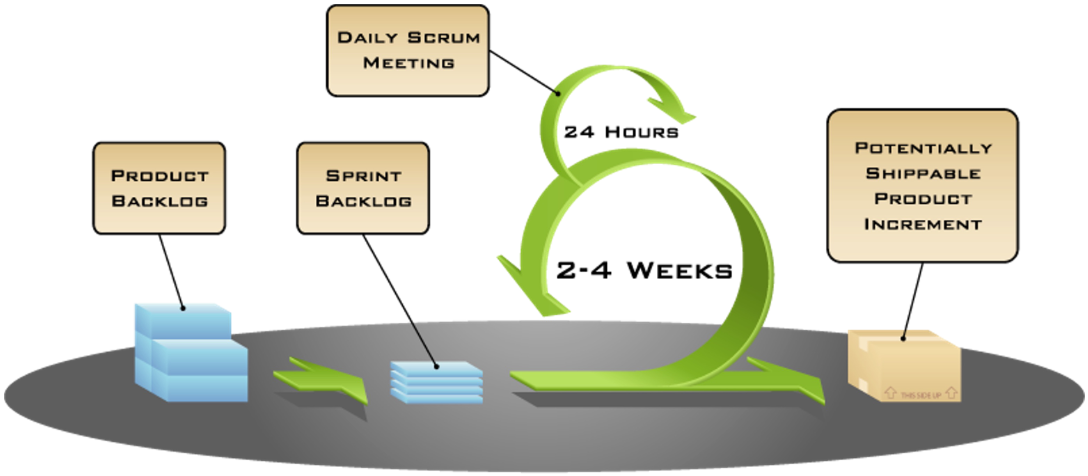
\includegraphics[width=0.9\textwidth]{images/Scrum1.png} \\ \\
    \end{tabular}
\end{center}

\subsection{Ruoli}

\subsubsection{Product Owner}
\begin{itemize}
    \item Definisce le caratteristiche del prodotto
    \item Rappresenta il desiderio del committente
    \item Decide date e contenuto del rilascio
    \item È responsabile della redditività del prodotto (ROI)
    \item Definisce le priorità delle caratteristiche del prodotto in base al valore che il mercato gli attribuisce
    \item Adegua le caratteristiche e la priorità ad ogni iterazione, secondo quanto necessario
    \item Responsabile che il Product Backlog sia chiaro e ordinato
    \item Accetta o rifiuta i risultati del lavoro
\end{itemize}

\subsubsection{Scrum Master}
\begin{itemize}
    \item Rappresenta la conduzione del progetto
    \item Responsabile dell'adozione dei valori e delle pratiche Scrum
    \item Rimuove gli ostacoli
    \item Si assicura che il gruppo di lavoro sia pienamente operativo e produttivo
    \item Favorisce una stretta cooperazione tra tutti i ruoli e le funzioni
    \item Protegge il gruppo di lavoro da interferenze esterne
    \item Servant leader: aiuta Product Owner e Team di sviluppo condividendo la gestione e le decisioni con il team
\end{itemize}

\subsubsection{Development Team}
\begin{itemize}
    \item Tipicamente 5-9 persone
    \item Responsabili di realizzare l'incremento in conformità alla Definition of Done
    \item Competenze trasversali (cross functional): programmatori, tester, progettisti di user experience, ...
    \item Membri di progetto dovrebbero lavorare full-time
    \item Possono esserci eccezioni (e. amministratori di database)
    \item Il gruppo di lavoro si auto-organizza: idealmente senza titoli, ma in rari casi può essere una possibilità
\end{itemize}

\newpage
\subsection{Eventi}

\subsubsection{Sprint Planning}
\begin{itemize}
    \item È un evento "Time boxed” di ~8h per Sprint di 1 mese
    \item Cosa può essere realizzato durante lo Sprint? Il Team seleziona dal product backlog gli item che può impegnarsi a completare
    \item Viene creato lo Sprint backlog collaborativamente da tutto il team
    \item Vengono identificate le Task, e ciascuno di questi viene stimato (1-16 ore)
    \item Come completare il backlog?
    \item Decomposizione delle User Story
\end{itemize}
\begin{center}
    \begin{tabular}{c}
        \\ 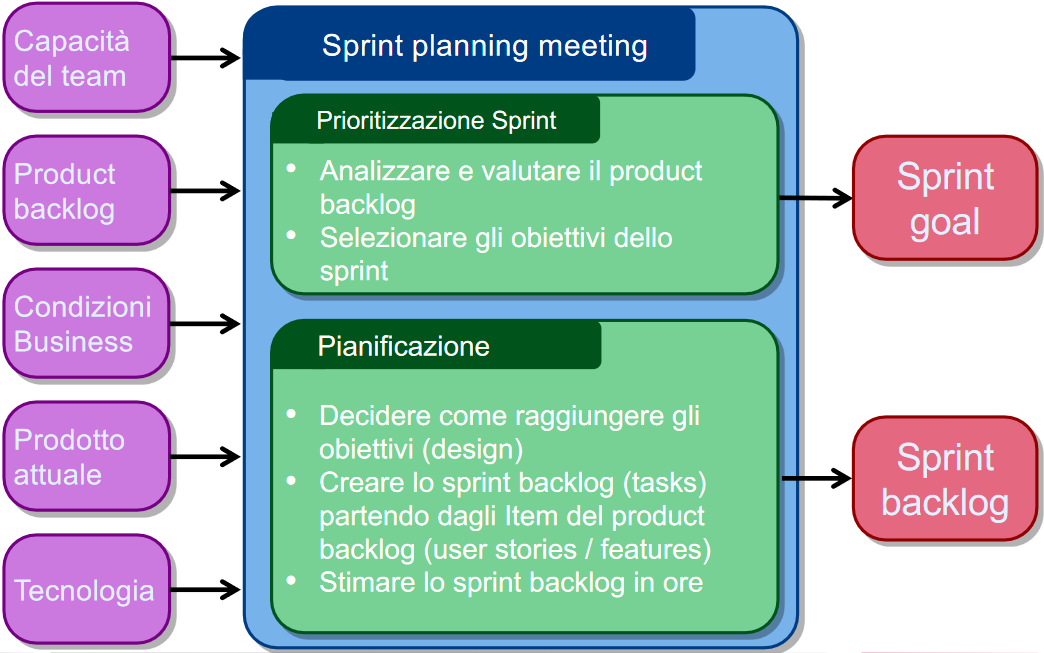
\includegraphics[width=0.9\textwidth]{images/Scrum2.png} \\ \\
    \end{tabular}
\end{center}

\subsubsection{Daily Scrum Meeting}
\begin{itemize}
    \item Incontro giornaliero di 15 minuti, fatto in piedi
    \item Non per la soluzione di problemi, ma per sincronizzarsi su quanto fatto e pianificare la giornata per il raggiungimento dello Sprint Goal
    \item Si aggiorna la scrumboard
    \item Aiuta ad evitare altre riunioni non necessarie
    \item In caso può partecipare anche il Product Owner
    \item Domande:
    \begin{itemize}
        \item Cosa hai fatto ieri?
        \item Cosa farai oggi?
        \item C'è qualcosa che ti impedisce di farlo?
    \end{itemize}
\end{itemize}

\subsubsection{Sprint Review}
\begin{itemize}
    \item Time boxed: ~4h per Sprint di 1 Mese
    \item Il gruppo di lavoro presenta ciò che ha realizzato durante lo sprint
    \item Viene validato e accettato quanto realizzato
    \item Tipicamente in forma di demo delle nuove caratteristiche o dell'architettura sottostante
    \item Informale:
    \begin{itemize}
        \item Regola delle 2 ore per la preparazione
        \item Niente slide
    \end{itemize}
    \item Partecipa tutto il gruppo
    \item Tutti sono invitati (anche gli esterni)
\end{itemize}

\subsubsection{Sprint Retrospective}
\begin{itemize}
    \item Si celebra dopo la Sprint Review e prima del prossimo Sprint Planning
    \item Time boxed: 3 ore per Sprint di 1 mese
    \item Si valuta ciò che sta funzionando e ciò che non sta funzionando
    \begin{itemize}
        \item Come migliorare la qualità del prodotto?
        \item La Definition of Done è appropriata?
        \item Che miglioramenti possiamo apportare al prossimo Sprint?
    \end{itemize}
    \item Partecipa tutto il gruppo di lavoro:
    \begin{itemize}
        \item Scrum Master
        \item Product Owner
        \item Development Team
    \end{itemize}
\end{itemize}

\subsection{Artefatti}

\subsubsection{Product Backlog}
\begin{itemize}
    \item I requisiti, funzionalità, miglioramenti, fix da realizzare nei prossimi rilasci
    \item Una lista di tutti i “desiderata”
    \item Idealmente espressa in modo che ciascun elemento ha valore per gli utenti o I clienti del prodotto
    \item Priorità assegnate dal Product Owner mentre il Dev. Team stima ogni item
    \item Priorità rivalutate all'inizio di ogni sprint con il Development Team
    \item Raffinamento continuo, è una lista dinamica che evolve con il prodotto
\end{itemize}

\begin{mdframed}
    User Stories: Item che compongono il Product Backlog e andranno scomposte in Task
\end{mdframed}

\subsubsection{Sprint Backlog}
\begin{itemize}
    \item Ogni componente del Development Team si sceglie qualcosa da fare
    \item La stima del lavoro rimanente è aggiornata ogni giorno
    \item Ogni membro del gruppo di lavoro può aggiungere, cancellare o modificare parti dello sprint backlog
    \item Il lavoro da svolgere durante lo sprint “emerge”
    \item Se il lavoro non è chiaro, definire un elemento dello sprint backlog con una stima temporale più ampia, e decomporlo successivamente
    \item Aggiornare il lavoro rimanente man mano che diventa più chiaro
    \item Massima visibilità della scrumboard
\end{itemize}

\subsubsection{Definition of Done}
\begin{itemize}
    \item Il minimo set di attività per definire che un'attività è completata
    \item Può variare per gruppo di lavoro
    \item Deve essere bene chiaro per tutti i membri del gruppo di lavoro
    \item È utilizzato per verificare se un'attività è da ritenersi completata
\end{itemize}

\subsubsection{Acceptance Criteria}
\begin{itemize}
    \item Permette di confermare se la storia è completa e funziona come voluto
    \item Frasi semplici condivise da Product Owner e Development Team
    \item Possono essere incluse con la User Story
    \item Rimuovono l'ambiguità dei requisiti
\end{itemize}

\newpage